% LTeX: language=es, en

\documentclass{beamer}
\usepackage[spanish, mexico]{babel}
\usepackage[T1]{fontenc}
\usepackage[style=authortitle,backend=bibtex]{biblatex}
\addbibresource{biblio.bib}
\usepackage{csquotes}
\usepackage{graphicx}
\usepackage{url}
\graphicspath{img/}

\usetheme{moloch}
\setbeamertemplate{footline}[frame number]

\title{Desarrollo sustentable}
\subtitle{Problemas sociales}
\author{Abraham Olivetti}
\institute{UTR}

\begin{document}

\frame{
\maketitle
}


\section{Preámbulo}

\frame{
\frametitle{El amanecer de una época}
\begin{figure}
\centering
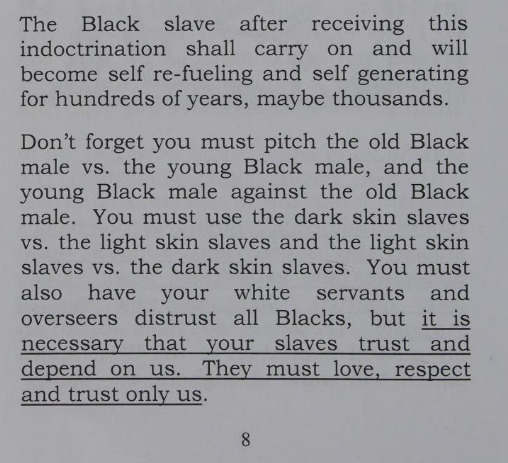
\includegraphics[width=0.5\linewidth]{img/lynch.jpeg}
\caption{La guía de Willie Lynch}
\label{fig:lynch}
\end{figure}
}

\frame{
\frametitle{El amanecer de una época}
\begin{figure}
\centering
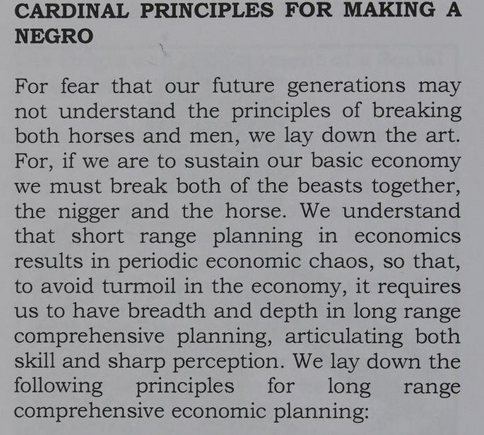
\includegraphics[width=0.5\linewidth]{img/lynchhorse.png}
\caption{La guía de Willie Lynch}
\label{fig:horse}
\end{figure}
}


\frame{
\frametitle{El amanecer de una época 2}
\begin{figure}
\centering
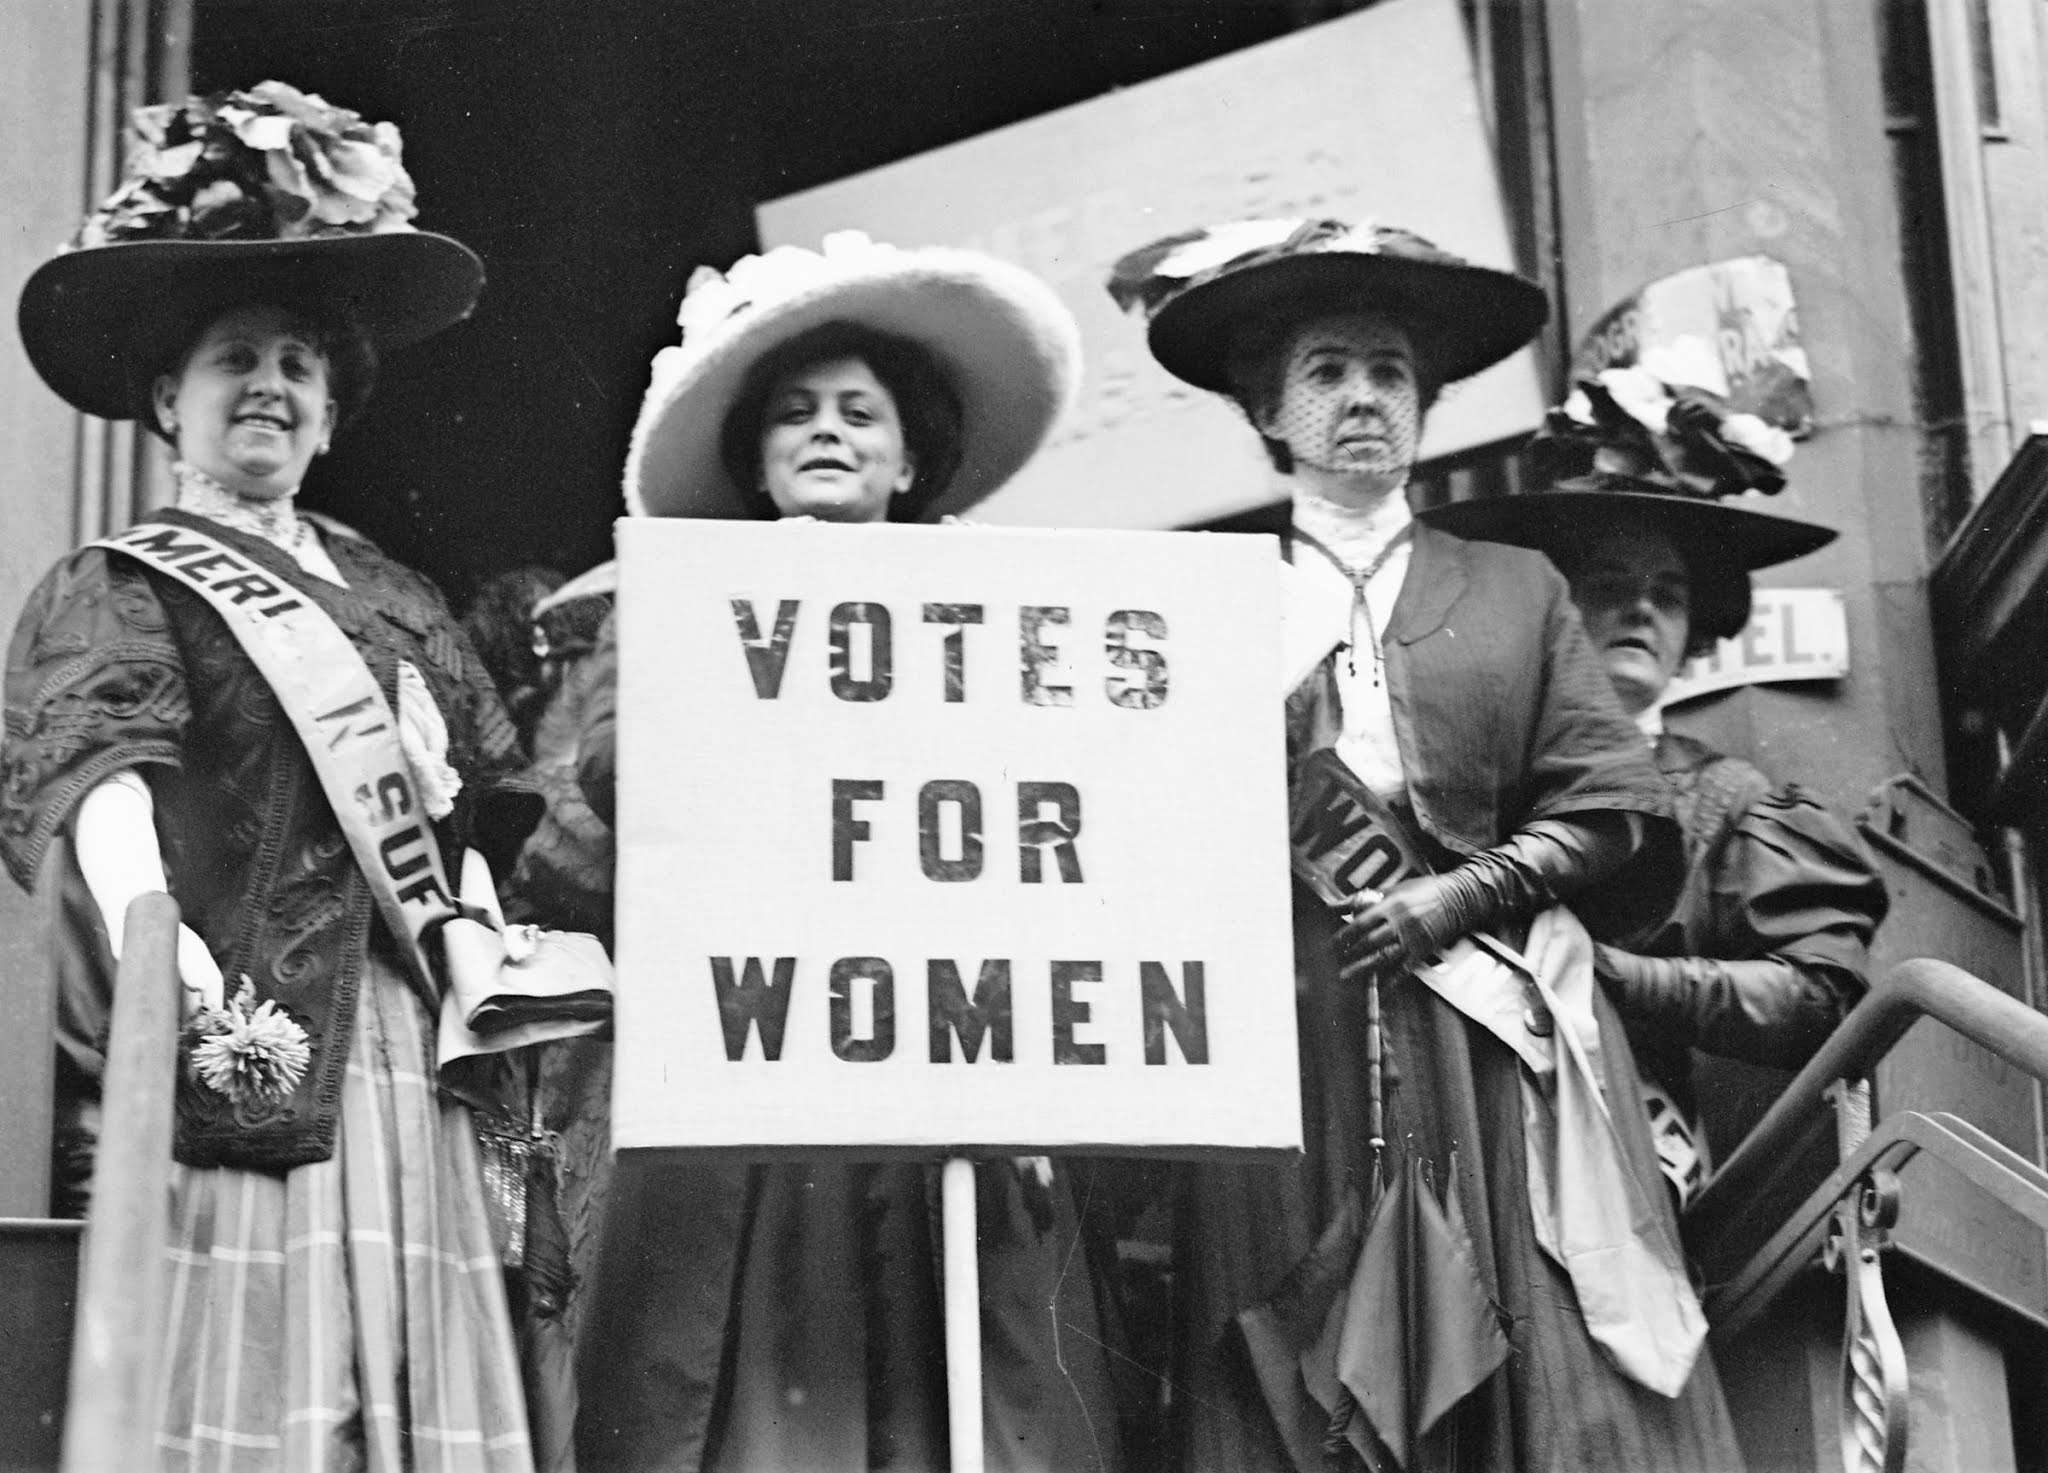
\includegraphics[width=0.7\linewidth]{img/sufrragio.jpg}
\caption{Sufragistas}
\label{fig:sufragio}
\end{figure}
}


\frame{
\frametitle{Diferentes condiciones sociales}
\begin{figure}
\centering
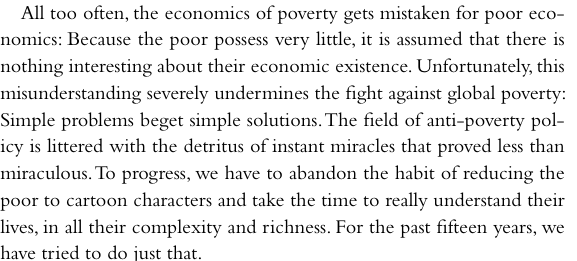
\includegraphics[width=0.9\linewidth]{img/cliches.png}
\caption{Los clichés}
\label{fig:clich}
\end{figure}
}


\frame{
\frametitle{El amanecer de \emph{nuestra} era}
\begin{itemize}
\item Con lo anterior, quiero enfatizar que las desigualdades sociales no son fenómenos de la historia antigua del ser humano
\pause
\item Aún tenemos fuertes brechas sociales.
\end{itemize}
}


\begin{frame}[standout]
865 millones de personas sobrevivieron con 36 centavos de dólar al día en 2005
\end{frame}


\frame{
\frametitle{¿Qué implica?}
\begin{itemize}
\pause
\item Desigualdad en la información
\pause
\item Desigualdad en la salud
\pause
\item Desigualdad educativa
\end{itemize}
}


\frame{
\frametitle{Nuestros propios sesgos}
\begin{quote}
    Food shortages in Malawi are affecting more than 3 million children;
    In Zambia, severe rainfall deficits have resulted in a 42\% drop in maize production from 2000. 
    As a result, an estimated 3 million Zambians face hunger; 
    Four million Angolans --tne third of the population-- have been forced to flee their homes;
    More than 11 million people in Ethiopia need immediate food assistance. 
\end{quote}
}


\frame{
\frametitle{``Mismo'' caso}
\begin{quote}
    Rokia, a 7-year-old girl from Mali, Africa, is desperately poor and faces a threat of severe hunger or even starvation.
    Her life will be changed for the better as a result of your financial gift. With your support, and the support of other caring sponsors, Save the Children will work with Rokia's family and other members of the community to help feed her, provide her with education, as well as basic medical care and hygiene education. 
\end{quote}
}


\frame{
\frametitle{Empezando}
\begin{itemize}
\pause
\item Comenzando por reconocer nuestros propios prejuicios
\pause
\item No debería sorprendernos que el segundo anuncio haya recabado más fondos
\pause
\item ¿Alguien quiere apostar por qué?
\end{itemize}
}


\section{Outline}


\frame{
\frametitle{Sugiero}
\begin{enumerate}

\pause
\item Que revisemos en qué consiste el \emph{contrato social}
\pause
\item Hablemos de algunas desigualdades sociales
\pause 
\item Revisemos qué soluciones se han ofrecido y cuáles han sido exitosas
\pause
\item Revisemos cómo surgen las desigualdades
\pause
\item Repasemos brevemente nuestros propios sesgos implícitos
\pause
\item Culminemos en especular qué papel juega la empatía en todo este esquema
\end{enumerate}
}

\section{Curso intensivísimo de filosofía moral}

\frame{
\frametitle{Supongo}
\begin{itemize}
    \pause
    \item Creo que todas aquí estamos de acuerdo que hay acciones \emph{moralmente buenas} y acciones \emph{moralmente malas}
    \pause
    \item Hemos discutido una buena variedad de temas para que también estemos de acuerdo con que es muy complicado trazar una línea clara entre ambas.
\end{itemize}
}


\frame{
\frametitle{Supongo también}
\begin{itemize}
    \pause
    \item Nos hemos respetado intelectualmente como para suponer que todas podemos participar en el juego de \emph{dar y recibir razones.}
\end{itemize}
}


\frame{
\frametitle{Cuestiones ``centrales''}
\begin{itemize}
    \pause
    \item ¿Qué hace que algo sea una acción buena$/$mala, justa$/$injusta?
    \pause
    \item ¿Es plausible el relativismo moral?
    \pause
    \item ¿Cuál es la base de las afirmaciones morales?
\end{itemize}
}


\begin{frame}[standout]
No podemos discutir todo esto porque no es una clase de filosofía moral
\end{frame}


\frame{
\frametitle{Es por ello}
\begin{itemize}
\item Les pedí que adoptáramos al \emph{contractualismo} como un marco bajo el cuál podemos analizar los desafíos que nos ocupan.
\end{itemize}
}


\frame{
\frametitle{También}
\begin{itemize}
\pause
\item Les pedí además que pensáramos a este contrato en términos de \emph{lo que nos debemos unos a otros}
\pause
\item Esto tiene dos propósitos: primero, que podamos responder a las preguntas anteriores sin tantos enredos;
segundo, que me voy a aprovechar que la frase ``lo que nos debemos unos a otros'' es polisémica.
\end{itemize}
}

\section{Nuestra idea de justicia}

\frame{
\frametitle{Me refiero}
\begin{itemize}
    \pause
    \item Quiero decir que es polisémica porque tenemos dos caras de una moneda. 
    \pause
    \item Por un lado, la teoría filosófica de Scanlon \parencite{scanlon} que aparece en su libro \emph{What We Owe to Each Other}
    \pause
    \item Por otro lado, la literatura en torno a las políticas de igualdad que se han discutido recientemente, englobadas en el libro \emph{What We Owe Each Other} de Shafik \parencite{shafik2021we}
\end{itemize}
}


\frame{
\frametitle{Confesé}
\begin{itemize}
\pause
\item No podemos revisar a detalle la teoría de Scanlon.
\pause
\item Entonces van a tener que creerme cuando les hable del libro de Scanlon (el fulano sigue vivo, le pueden escribir si quieren.)
\end{itemize}
}


\subsection{Contractualismo: al menos lo de Scanlon}

\frame{
\frametitle{Contractualismo}
\begin{itemize}
\pause
\item Les sugerí que para finalidades del curso, adoptemos esta teoría política.
\pause
\item Si es verdad lo que señalamos, entonces este contrato social debe tener serias modificaciones
\end{itemize}
}

\frame{
\frametitle{Atención}
\begin{itemize}
\pause
    \item Quiero enfatizar que estamos \emph{adoptando} la teoría del contrato social que nos presenta Scanlon
    \pause
    \item Porque el contractualismo tiene sus propios problemas teóricos.
\end{itemize}
}

\begin{frame}[standout]
Las siguientes son citas clave
\end{frame}


\frame{
\frametitle{Una cita}
\begin{quote}
If we could characterize the method of reasoning through which we arrive at judgments of right and wrong, and could explain why there is good reason to give judgments arrived at in this way the kind of importance that moral judgments are normally thought to have, then we
would, I believe, have given a sufficient answer to the question of the subject matter of right and wrong as well. 
No interesting question would remain about the ontology of morals --for example, about the metaphysical status of moral facts. \parencite{scanlon}
\end{quote}
}


\frame{
\frametitle{Scanlon}
\begin{quote}
    When I ask myself what reason the fact that an action would be wrong provides me with not to do it, my answer is that such an action would be one that I could not justify to others on grounds I could expect them to accept. \parencite{scanlon}
\end{quote}
}


\frame{
\frametitle{The game of giving reasons}
\begin{quote}
    It holds that thinking about right and wrong is, at the most basic level, thinking about what could be justified to others on grounds that they, if appropriately motivated, could not reasonably reject. \parencite{scanlon}
\end{quote}
}


\section{Cómo lidiar con la desigualdad}

\frame{
\frametitle{Desigualdad}
\begin{itemize}
\pause
\item ¿Igualdad de oportunidades?
\pause
\item Pensemos en la analogía con la línea de salida de una carrera.
\pause
\item Digamos que si cualquier persona quiere ser nadadora olímpica, se asegure que cualquiera pueda hacerlo.
\end{itemize}
}


\frame{
\frametitle{¿Qué \emph{deberíamos} incluir?}
\begin{itemize}
\pause
\item Trabajo
\pause
\item Vivienda
\pause
\item Alimento
\pause
\item Educación
\pause
\item ¿Deberíamos?
\end{itemize}
}

\frame{
\frametitle{¿Por qué deberíamos?}
\begin{itemize}
\pause
\item La respuesta obvia es que \emph{deberíamos} dar estos servicios, porque son necesarios para vivir.
\pause
\item Es decir que si estas necesidades no están cubiertas, entonces debemos pagar --por ejemplo-- comida. En lugar de pagar, digamos, internet.
\end{itemize}
}

\begin{frame}[standout]
Si dejamos que estas necesidades básicas participen en el mercado (venta y compra), las consecuencias son aterradoroas
\end{frame}

\frame{
\frametitle{Desconfianza}
\begin{itemize}
\item Aún así hay cierta reserva social en los apoyos económicos y en cómo se distribuye la riqueza
\end{itemize}
}



\section{Bienes no dispuestos a venta}

\frame{
\frametitle{James Tobin}
\begin{itemize}
\item Deberíamos separar nuestra idea de justicia social de la eficiencia mercantil.
\pause
\item La apuesta era que si los mercados son eficientes, entonces la justicia \emph{sale gratis}
\end{itemize}
}

\frame{
\frametitle{Justicia y eficiencia mercantil}
\begin{figure}
\centering
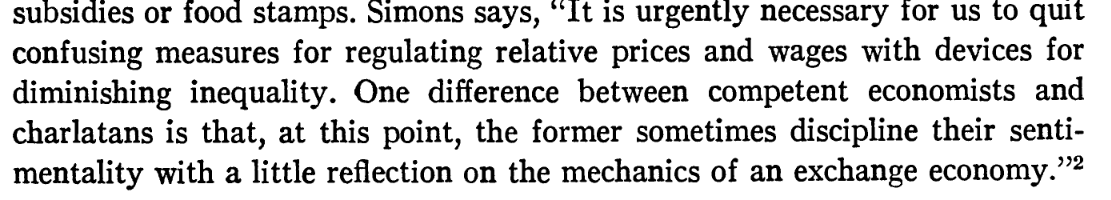
\includegraphics[width=0.9\linewidth]{img/charlatans.png}
\caption{Los dos ministerios}
\label{fig:charla}
\end{figure}
}

\frame{
\frametitle{James Tobin}
\begin{figure}
\centering
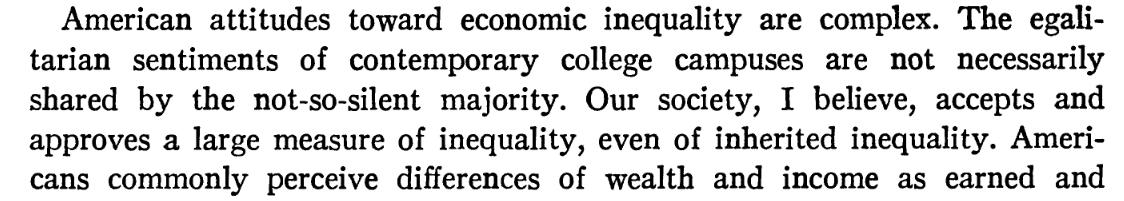
\includegraphics[width=0.9\linewidth]{img/tobin1.png}
\caption{\cite{tobinlimit}}
\label{fig:tobin1}
\end{figure}
}

\frame{
\frametitle{James Tobin}
\begin{figure}
\centering
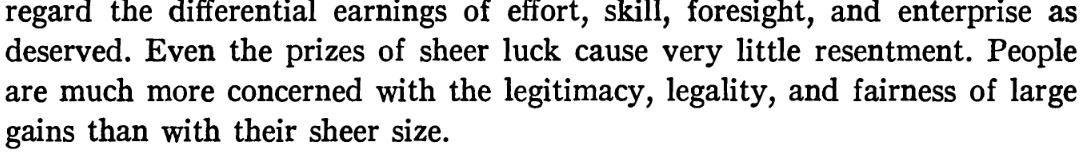
\includegraphics[width=0.9\linewidth]{img/tobin2.png}
\caption{\cite{tobinlimit}}
\label{fig:tobin2}
\end{figure}
}


\begin{frame}
\frametitle{Tobin}
    \begin{enumerate}
    \item El argumento es simple y elegante
        \begin{enumerate}
        \item La distribución de recursos económicos no está funcionando
            \begin{enumerate}
            \item Principalmente porque los mercados no son eficientes
            \end{enumerate}
    \item Si la distribución de recursos económicos no está funcionando, entonces \emph{deberíamos} distribuir bienes
        \begin{enumerate}
        \item \emph{Deberíamos}, principalmente, porque estamos de acuerdo de que hay bienes básicos (aquí es donde me parece entra el acuerdo)
        \end{enumerate}
  \item \emph{Deberíamos} distribuir bienes, entonces separemos a la eficiencia mercantil de la justicia social
  \end{enumerate}
  \end{enumerate}
\end{frame}


\begin{frame}[standout]
Dios santo, esto es demasiado obvio como para que valga la pena mencionarlo.
\end{frame}

\frame{
\frametitle{LDE}
\begin{figure}
\centering

\includegraphics[width=0.9\linewidth]{img/dios1.png}
\caption{1970}
\label{fig:dios}
\end{figure}
}

\frame{
\frametitle{LDE}
\begin{figure}
\centering

\includegraphics[width=0.9\linewidth]{img/dios2.png}
\caption{1970}
\label{fig:santo}
\end{figure}
}


\frame{
\frametitle{Pensemos en tres casos}
    \begin{itemize}
    \pause
    \item Salud
    \pause
    \item Vivienda
    \pause
    \item Educación
    \end{itemize}
}

\frame{
\frametitle{Sandel}
\begin{figure}
\centering

\includegraphics[width=0.9\linewidth]{img/sandel1.png}
\caption{Lo que el dinero no puede comprar}
\label{fig:sandel1}
\end{figure}
}

\frame{
\frametitle{Sandel}
\begin{figure}
\centering
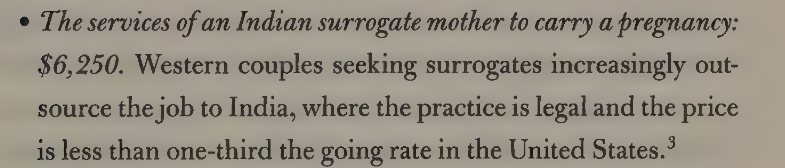
\includegraphics[width=0.9\linewidth]{img/sandel2.png}
\caption{Lo que el dinero no puede comprar}
\label{fig:sandel2.png}
\end{figure}
}

\frame{
\frametitle{Sandel}
\begin{figure}
\centering

\includegraphics[width=0.9\linewidth]{img/sandel3.png}
\caption{Lo que el dinero no puede comprar}
\label{fig:sandel3}
\end{figure}
}


\frame{
\frametitle{Sandel}
\begin{figure}
\centering
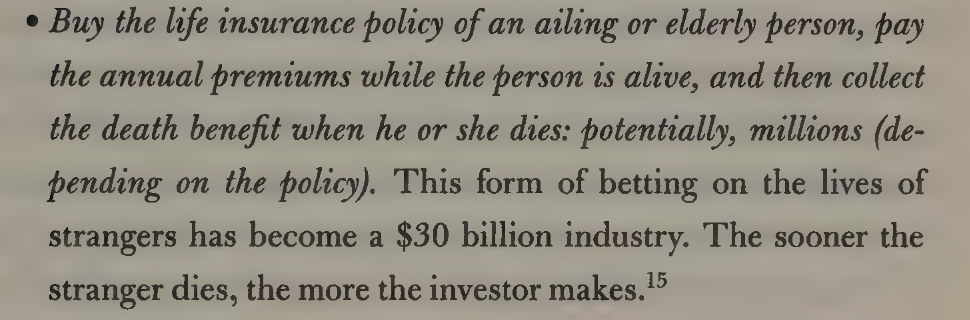
\includegraphics[width=0.9\linewidth]{img/sandel4.png}
\caption{Lo que el dinero no puede comprar}
\label{fig:sandel4}
\end{figure}
}

\frame{
\frametitle{Sandel}
\begin{figure}
\centering
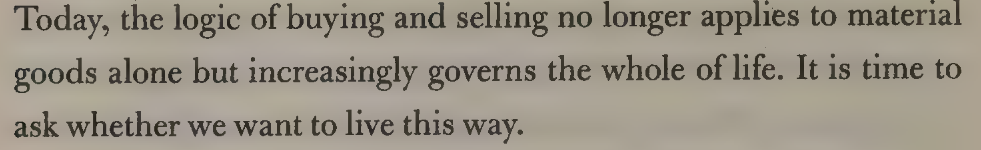
\includegraphics[width=0.9\linewidth]{img/sandel5.png}
\caption{Lo que el dinero no puede comprar}
\label{fig:sandel5}
\end{figure}
}

\frame{
\frametitle{Sandel}
\begin{figure}
\centering
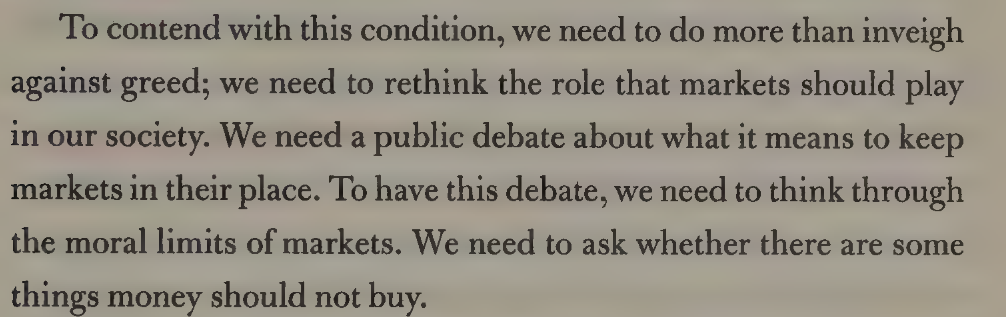
\includegraphics[width=0.9\linewidth]{img/sandel6.png}
\caption{Lo que el dinero no puede comprar}
\label{fig:sandel6}
\end{figure}
}


\frame{
\frametitle{Pero todavía no está asegurada}
    \begin{itemize}
    \item Sigamos con nuestra línea de carrera
    \pause
    \item Hay personas que pueden tropezar
    \pause
    \item Por lo que la falta de habilidad es \emph{sólo} un factor.
    \end{itemize}
}

\begin{frame}[standout]
El problema radica en afirmar que una vez que las oportunidades \emph{ex ante} están aseguradas, las oportunidades \emph{ex post} son irrelevantes.
\end{frame}

\frame{
\frametitle{\emph{ex post} \& \emph{ex ante}}
\begin{quote}
    Those who think inequality of outcome is irrelevant regard concern for \emph{ex post} outcomes as illegitimate and believe that, once a level playing field for the race of life has  been established, we should not enquire into the outcomes. \parencite{atkinson2015inequality}
\end{quote}
}

%\section{Confesión}

%\frame{
%\frametitle{Qué está pasando}
%\begin{itemize}
%    \item Creo que hay algo en lo que he fallado hasta ahora
%    \pause
%    \item Me refiero a que creo que no he logrado convencerles de la importancia de estos temas
%\end{itemize}
%}


%\frame{
%\frametitle{Nuestros temas pasados}
%\begin{itemize}
%    \item Las primeras semanas revisamos la ``ciencia'' básica del cambio climático
%    \pause
%    \item Revisamos el problema del efecto invernadero.
%    \pause
%    \item Señalamos algunas de sus causas
%    \pause
%    \item Exploramos algunas de sus consecuencias
%\end{itemize}
%}


%\frame{
%\frametitle{Consecuencias sociales}
%\begin{itemize}
%    \item Repasamos brevemente cuáles son las consecuencias sociales de nuestra interacción con el ambiente
%    \pause
%    \item Me interesaba que nos centráramos en las consecuencias sociales porque estos problemas han dejado de ser debates académicos
%    \pause
%    \item Han dejado de ser debates académicos y se han convertido en una necesidad social
%\end{itemize}
%}

%\frame{
%\frametitle{Consecuencias para los desfavorecidos}
%\begin{itemize}
%    \item Si ustedes revisan cualquier manual oficial sobre la enseñanza de esta materia, sabrán que se esperan demasiadas cosas para sólo un curso.
%\end{itemize}
%}

%\frame{
%\frametitle{Por ejemplo}
%\begin{quote}
%Education for sustainable development (ESD) gives learners of all ages the knowledge, skills, %values and agency to address interconnected global challenges including climate change, loss of %biodiversity, unsustainable use of resources, and inequality. \cite{UNESCO_2024}
%\end{quote}
%}

%\frame{
%\frametitle{Pero en la medida}
%\begin{itemize}
%\item de lo posible, vamos a tratar con cierto detalle el problema de la desigualdad
%\end{itemize}
%}


\section{El estado de la teoría económica actual}

\frame{
\frametitle{Deuda}
\begin{figure}
\centering

\includegraphics[width=0.7\linewidth]{img/debt.jpg}
\caption{David Graeber}
\label{fig:deuda}
\end{figure}
}

\frame{
\frametitle{Deuda}
\begin{figure}
\centering
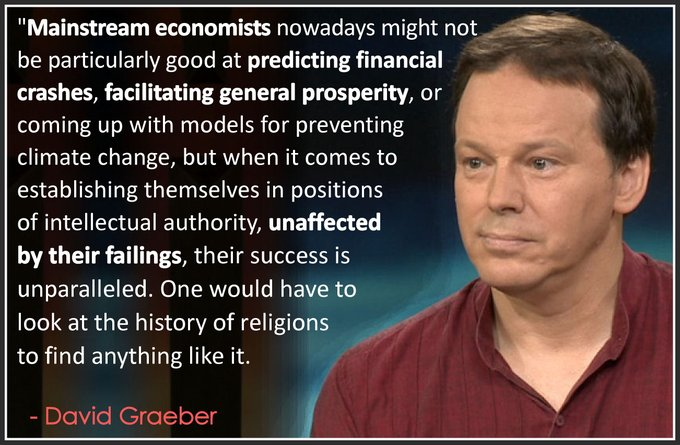
\includegraphics[width=0.7\linewidth]{img/graeber.jpg}
\caption{David Graeber}
\label{fig:graeber}
\end{figure}
}

\frame{
\frametitle{Títulos y eso}
\begin{itemize}
    \item Lo sé, no soy economista.
    \pause
    \item Pero creo que tengo el conocimiento suficiente de economía y estadística como para revisar literatura contemporánea al respecto.
    \pause
    \item Al menos trato de traerles información de personas que todavía siguen vivas.
\end{itemize}
}


\frame{
\frametitle{Se suele}
    \begin{itemize}
    \item Señalar que nuestra función de utilidad siempre responde a los beneficios propios
    \pause
    \item Pero en algunas ocasiones, las personas están dispuestas a cooperar
    \end{itemize}
    }


\section{Brevísima caraterización}

\frame{
\frametitle{Hasta aquí}
\begin{itemize}
    \item Hemos visto algunas de las consecuencias de empatar la \emph{eficiencia mercantil} con \emph{la igualdad de oportunidades}
    \pause
    \item Hemos revisado cómo podríamos cerrar la brecha económica
    \pause
    \item Sabemos que la simple ayuda monetaria no nos asegura la \emph{justicia}
\end{itemize}
}


\frame{
\frametitle{Tenemos, por ejemplo}
\begin{itemize}
    \item Personas que no pueden tener un excedente (barrera económica)
    \pause
    \item Personas que viven a largas distancias de las zonas donde se concentran los intercambios mercantiles (barrera geográfica)
    \pause
    \item Personas a quienes se les impide acceder a bienes y servicios (barrera cultural)
\end{itemize}
}

\frame{
\frametitle{Nuestra apuesta}
\begin{itemize}
    \item Fue que deberíamos asegurar la igualdad de oportunidades para todos los ciudadanos
    \pause
    \item Que incluso si quieren ceder sus derechos voluntariamente, no sea posible.
\end{itemize}
}


\frame{
\frametitle{Además}
\begin{itemize}
    \pause
    \item Se ha discutido recientemente que la economía \emph{debería} estar informada por la filosofía moral \parencite{sandel1998money, atkinson2009economics}
\end{itemize}
}


\frame{
\frametitle{Deuda}
\begin{figure}
\centering
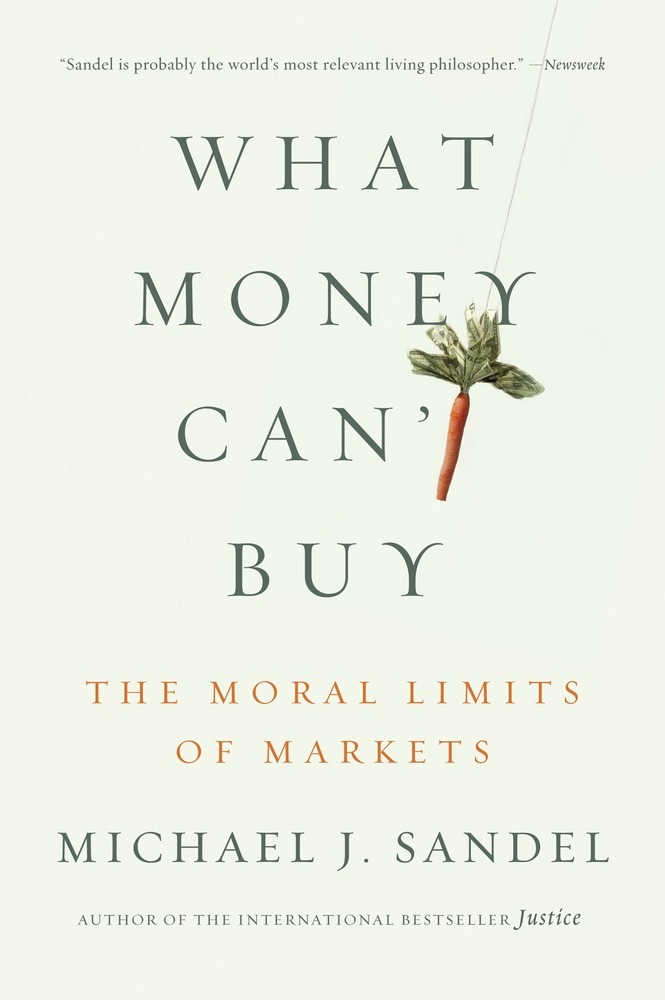
\includegraphics[width=0.4\linewidth]{img/sandel.jpg}
\caption{Michael Sandel}
\label{fig:cantbuy}
\end{figure}
}


\frame{
\frametitle{Deuda}
\begin{figure}
\centering

\includegraphics[width=0.9\linewidth]{img/asmoral.png}
\caption{Anthony Atkinson}
\label{fig:moralsc}
\end{figure}
}

\frame{
\frametitle{Indicadores estructurales UE}
\begin{figure}
\centering
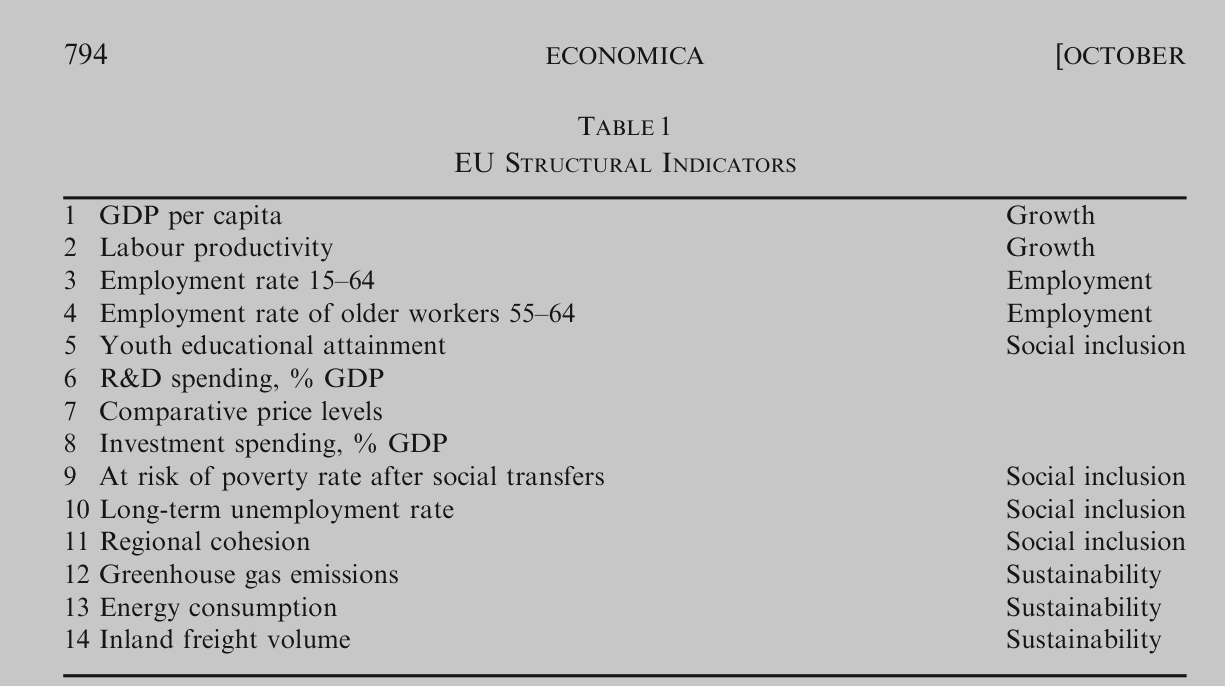
\includegraphics[width=0.9\linewidth]{img/indicestr.png}
\caption{Indicadores por categoría}
\label{fig:struct}
\end{figure}
}


\section{Brevísima caraterización}

\frame{
\frametitle{Hasta aquí}
\begin{itemize}
    \item Hemos visto algunas de las consecuencias de empatar la \emph{eficiencia mercantil} con \emph{la igualdad de oportunidades}
    \pause
    \item Hemos revisado cómo podríamos cerrar la brecha económica
    \pause
    \item Sabemos que la simple ayuda monetaria no nos asegura la \emph{justicia}
\end{itemize}
}


\begin{frame}
\frametitle{\emph{Laissez-Faire}}
\begin{itemize}
\pause
    \item Teoría económica que defiende la mínima intervención gubernamental en la economía.
    \pause
    \item Los mercados deben funcionar sin regulaciones estatales.
    \pause
    \item Las fuerzas de oferta y demanda se autorregulan, asignando los recursos eficientemente.
    \pause
    \item El interés propio de individuos y empresas conduce al crecimiento económico y bienestar general.
\end{itemize}
\end{frame}


\begin{frame}
\frametitle{Economía Keynesiana}
\begin{itemize}
    \pause
    \item La intervención del gobierno es esencial para estabilizar la economía.
    \pause
    \item La demanda agregada (gasto de consumidores, empresas y gobierno) es el motor principal del crecimiento económico.
    \pause
    \item En recesión, la insuficiente demanda puede generar desempleo.
    \pause
    \item El gobierno debe intervenir con gasto público o reducciones de impuestos para estimular la economía.
\end{itemize}
\end{frame}

\begin{frame}
\frametitle{Pero}
\begin{itemize}
\item Nuestros mercados no son eficientes.
\begin{itemize}
\item No hay competencia mercantil (monopolios)
\pause
\item Los humanos no calculamos adecuadamente la expectativa (debido a los varios sesgos)
\pause
\item Difícilmente tenemos información perfecta
\end{itemize}
\end{itemize}
\end{frame}



\frame{
\frametitle{Información}
\begin{quote}
Similarly, costly information explains why banks ration credit.
Why ration rather than simply charge higher interest rates to higher-risk borrowers?
Because often the only borrowers who will borrow at high rates are those who are the highest risk --and on whom, therefore, the lenders are most likely to lose. \parencite{econlibInformationJoseph}
\end{quote}
}

\frame{
\frametitle{Volatilidad}
 \begin{quote}
Thus, the characteristics of credit and equity markets --characteristics that can be explained by imperfect, costly, and asymmetric information-- help explain the volatility of the economy. \parencite{econlibInformationJoseph}
 \end{quote}
}


\frame{
\frametitle{Sen}
\begin{figure}
\centering
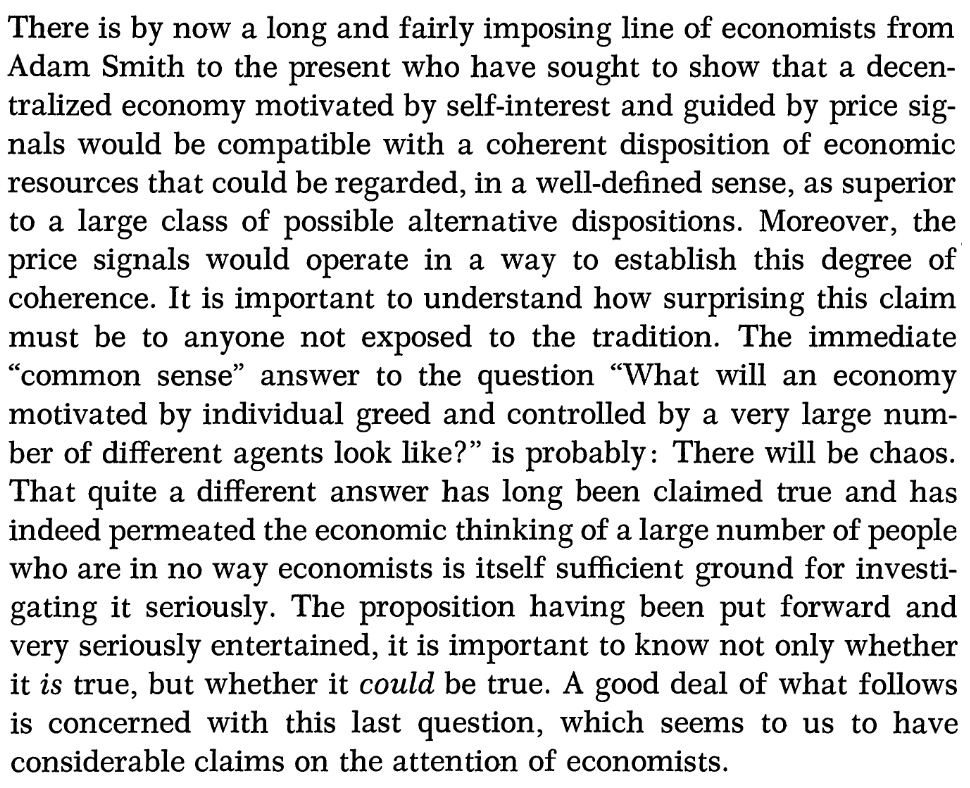
\includegraphics[width=0.9\linewidth]{img/chaos.png}
\caption{Rational fools}
\label{fig:chaos}
\end{figure}
}

\frame{
\frametitle{Sen}
\begin{figure}
\centering
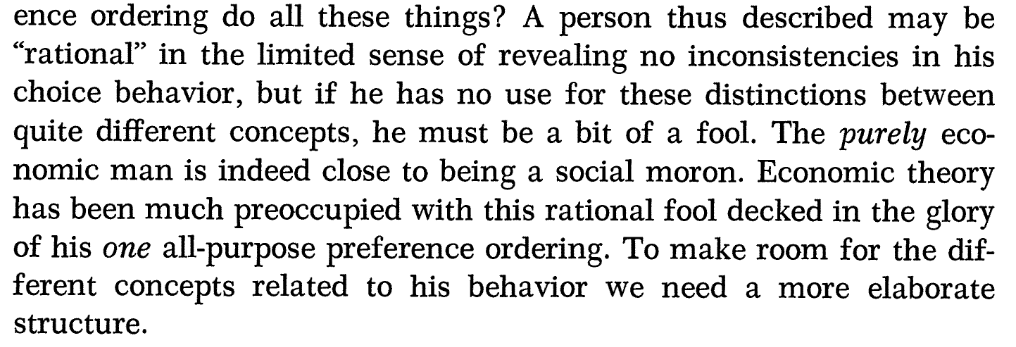
\includegraphics[width=0.9\linewidth]{img/bitfool.png}
\caption{Sen}
\label{fig:bitfool}
\end{figure}
}

\frame{
\frametitle{Sen}
\begin{figure}
\centering
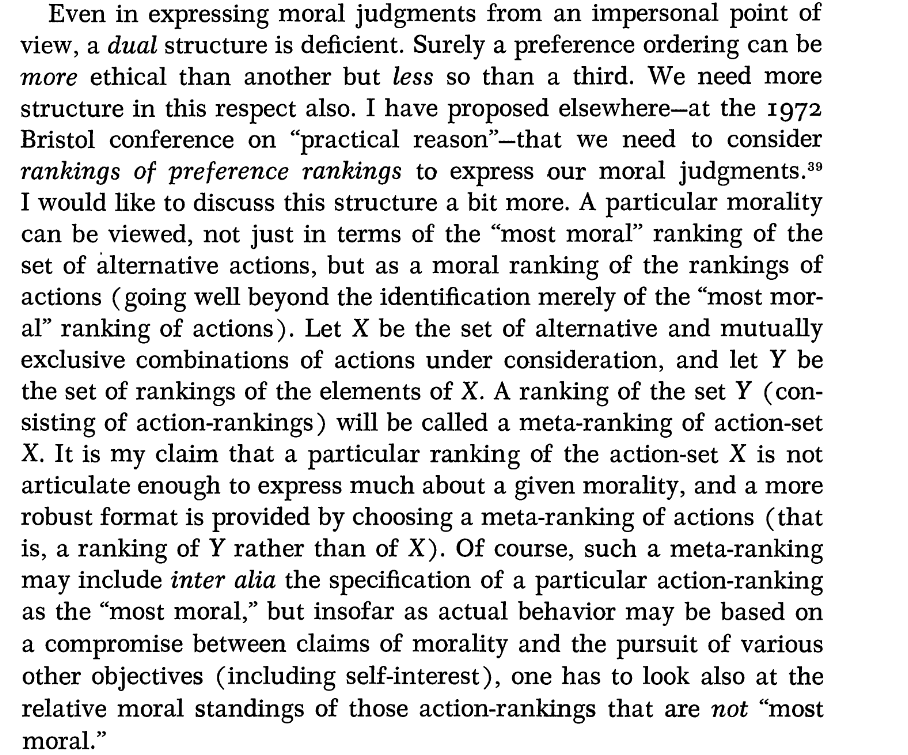
\includegraphics[width=0.9\linewidth]{img/theranking.png}
\caption{Rational fool}
\label{fig:therank}
\end{figure}
}

\frame{
\frametitle{Sen}
\begin{figure}
\centering
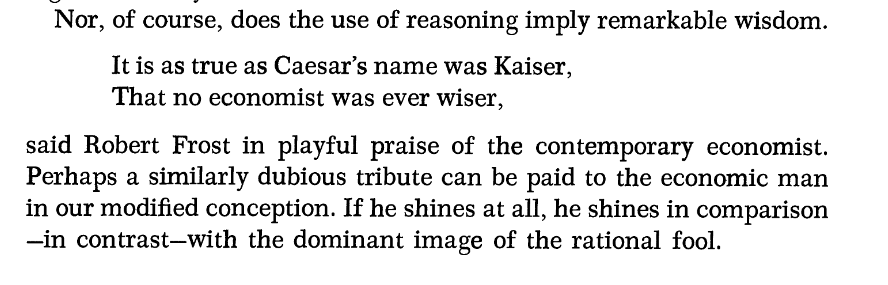
\includegraphics[width=0.9\linewidth]{img/rationalfool.png}
\caption{Rational fools}
\label{fig:ratiofoo}
\end{figure}
}




\frame{
\frametitle{Porque}
\begin{itemize}
\item Muchas \emph{injusticias} han sido parte del \emph{contrato social}
    \begin{itemize}
    \pause
    \item Ya la Grecia antigua tenía la figura del esclavo
    \pause
    \item Que era una figura estatal.
    \pause
    \item Preguntémonos ¿qué causa las desigualdades?
    \end{itemize}
\end{itemize}
}

\begin{frame}[standout]
Una vez entrando en el contrato social, cedemos ciertas libertades por el bien de la comunidad
\end{frame}



\begin{frame}[allowframebreaks]
\printbibliography
\end{frame}


\end{document}
